\subsection{Cyclic Groups}

Cyclic groups are fundamental building blocks in group theory. Every finite Abelian group can be decomposed into cyclic groups, so understanding their structure is essential.

\Definition{Cyclic Group}{
    A group $G$ is called a \textbf{cyclic group} if there exists an element $g \in G$ such that every element in $G$ can be expressed as $g^n$ for some integer $n$. \[ 
        G = \langle g \rangle = \{g^n \mid n \in \Z\}
    \]
    The element $g$ is called a \textbf{generator} of the group $G$.
}


%%%%%%%%%%%%%%%%%%%%%%%%%%%%%%%%%%%%%%%%%%%%
%  Elementary Properties of Cyclic Groups  %
%%%%%%%%%%%%%%%%%%%%%%%%%%%%%%%%%%%%%%%%%%%%

\subsubsection{Elementary Properties of Cyclic Groups}

\Theorem{}{
    Every cyclic group is Abelian.
}

\Proof{
    Let $G = \langle g \rangle$ be a cyclic group. If $g_1, g_2 \in G$, then $g_1 = g^r$ and $g_2 = g^s$ for some $r, s \in \Z$. Then \[
        g_1 g_2 = g^r g^s = g^{r+s} = g^{s+r} = g^s g^r = g_2 g_1
    \]
    so $G$ is Abelian.
}

\Note{
    The converse is false: not every Abelian group is cyclic. For instance, the Klein 4-group $V$ is Abelian but not cyclic.
}


%%%%%%%%%%%%%%%%%%%%%%%%%%%%
%  The Division Algorithm  %
%%%%%%%%%%%%%%%%%%%%%%%%%%%%

\subsubsection{The Division Algorithm}

\Theorem{Division Algorithm for $\Z$}{
    If $m$ is a positive integer and $n$ is any integer, then there exist unique integers $q$ (quotient) and $r$ (remainder) such that \[
        n = mq + r \qquad \text{where } 0 \leq r < m
    \]
}

\Note{
    The idea is simple: on the number line, $n$ either lands on a multiple of $m$ (then $r = 0$), or it falls between two consecutive multiples $qm$ and $(q+1)m$, and $r$ is the distance from $qm$ to $n$. This is the same long division taught in elementary school, formalized for all integers.
}

\Example{}{
    When $38$ is divided by $7$: since $35 = 7 \cdot 5$, we get $38 = 7(5) + 3$, so $q = 5$ and $r = 3$.

    When $-38$ is divided by $7$: since $-42 = 7(-6)$, we get $-38 = 7(-6) + 4$, so $q = -6$ and $r = 4$. Note that the remainder must be nonnegative.
}


%%%%%%%%%%%%%%%%%%%%%%%%%%%%%%%%
%  Subgroups of Cyclic Groups  %
%%%%%%%%%%%%%%%%%%%%%%%%%%%%%%%%

\subsubsection{Subgroups of Cyclic Groups}

\Theorem{}{
    A subgroup of a cyclic group is cyclic.
}

\Proof{
    Let $G = \langle a \rangle$ be a cyclic group and let $H \leq G$. If $H = \{e\}$, then $H = \langle e \rangle$ is cyclic. If $H \neq \{e\}$, then $a^n \in H$ for some $n \in \Z^+$ (if $a^{-n} \in H$, then $(a^{-n})^{-1} = a^n \in H$ too). Let $m$ be the smallest positive integer such that $a^m \in H$. We claim $H = \langle a^m \rangle$.

    Let $b \in H$. Since $b \in G = \langle a \rangle$, we have $b = a^n$ for some $n \in \Z$. By the division algorithm, $n = mq + r$ where $0 \leq r < m$. Then \[
        a^r = a^{n - mq} = a^n (a^m)^{-q}
    \]
    Since $a^n \in H$ and $a^m \in H$ (hence $(a^m)^{-q} \in H$), we get $a^r \in H$. But $m$ was the smallest positive integer with $a^m \in H$ and $0 \leq r < m$, so $r = 0$. Thus $n = mq$ and $b = a^n = (a^m)^q$, showing $b \in \langle a^m \rangle$.
}

\Corollary{}{
    The subgroups of $\Z$ under addition are precisely the groups $n\Z$ for $n \in \Z_{\geq 0}$, i.e., every subgroup of $\Z$ is of the form $\{nk \mid k \in \Z\}$ for some nonnegative integer $n$.
}


%%%%%%%%%%%%%%%%%%%%%%%%%%%%%%%%%%%%%%%%%%%
%  Greatest Common Divisor via Subgroups  %
%%%%%%%%%%%%%%%%%%%%%%%%%%%%%%%%%%%%%%%%%%%

\subsubsection{Greatest Common Divisor via Subgroups}

\Definition{Greatest Common Divisor}{
    Let $r$ be a positive integer and $s$ a nonneg. integer. The set \[
        H = \{nr + ms \mid n, m \in \Z\}
    \]
    is a subgroup of $\Z$ under addition (can be verified using the one-step test). Since every subgroup of $\Z$ is cyclic, $H = d\Z$ for some positive integer $d$. This $d$ is the \textbf{greatest common divisor} of $r$ and $s$, written $d = \gcd(r, s)$.
}

\Note[Bézout's Identity]{
    Since $d \in H$, we can write $d = nr + ms$ for some integers $n, m$. This is called \textbf{Bézout's identity}. \\
    Also, since $r = 1 \cdot r + 0 \cdot s \in H = d\Z$ and $s = 0 \cdot r + 1 \cdot s \in H = d\Z$, we see that $d$ divides both $r$ and $s$. Any common divisor of $r$ and $s$ must divide $nr + ms = d$, so $d$ is indeed the greatest such divisor.
}

\Note{
    Two positive integers $r$ and $s$ are \textbf{relatively prime} if $\gcd(r, s) = 1$. \\
    A useful fact: if $r$ and $s$ are relatively prime and $r \mid sm$, then $r \mid m$. This is because $1 = ar + bs$ for some $a, b \in \Z$, so $m = arm + bsm$, and $r$ divides both terms on the right.
}


%%%%%%%%%%%%%%%%%%%%%%%%%%%%%%%%%%%%
%  The Structure of Cyclic Groups  %
%%%%%%%%%%%%%%%%%%%%%%%%%%%%%%%%%%%%

\subsubsection{The Structure of Cyclic Groups}

\Theorem{Classification of Cyclic Groups}{
    Let $G = \langle a \rangle$ be a cyclic group.
    \begin{itemize}
        \item If $G$ has infinite order, then $G \cong \langle \Z, + \rangle$.
        \item If $G$ has finite order $n$, then $G \cong \langle \Z_n, +_n \rangle$.
    \end{itemize}
}

\Proof{
    \textbf{Case 1 (infinite order):} Define $\phi : \Z \to G$ by $\phi(n) = a^n$. We verify that $\phi$ is an isomorphism:
    \begin{itemize}
        \item \textbf{Homomorphism:} For $m, n \in \Z$, we have $\phi(m + n) = a^{m+n} = a^m a^n = \phi(m) \phi(n)$.
        \item \textbf{Injective:} If $\phi(n) = e$, then $a^n = e$. Since $G$ has infinite order, the only power of $a$ that equals $e$ is $a^0 = e$, so $n = 0$. Thus $\ker(\phi) = \{0\}$ and $\phi$ is injective.
        \item \textbf{Surjective:} For any $g \in G$, we have $g = a^k$ for some $k \in \Z$, so $\phi(k) = g$. Thus $\phi$ is surjective.
    \end{itemize}
    \textbf{Case 2 (finite order):} Let $n = |G|$. Define $\phi : \Z_n \to G$ by $\phi(k) = a^k$. We verify that $\phi$ is an isomorphism:
    \begin{itemize}
        \item \textbf{Homomorphism:} For $k, r \in \Z_n$, we have $\phi(k +_n r) = a^{k +_n r} = a^k a^r = \phi(k) \phi(r)$.
        \item \textbf{Injective:} If $\phi(k) = e$, then $a^k = e$. Since $G$ has order $n$, the smallest positive integer $m$ such that $a^m = e$ is $n$. Thus, if $0 < k < n$, then $a^k \neq e$. The only way for $a^k$ to equal $e$ is if $k = 0$ in $\Z_n$. Hence $\ker(\phi) = \{0\}$ and $\phi$ is injective.
        \item \textbf{Surjective:} For any $g \in G$, we have $g = a^k$ for some $k \in \Z_n$, so $\phi(k) = g$. Thus $\phi$ is surjective.
    \end{itemize}
}

\Note{
    This theorem tells us there is essentially only one cyclic group of each order (up to isomorphism): $\Z$ for infinite order, and $\Z_n$ for order $n$. We can visualize the elements of a finite cyclic group $\langle a \rangle$ of order $n$ as points evenly spaced around a circle, with multiplication corresponding to ``adding angles'' modulo $n$:
}

\begin{figure}[H]
    \centering
    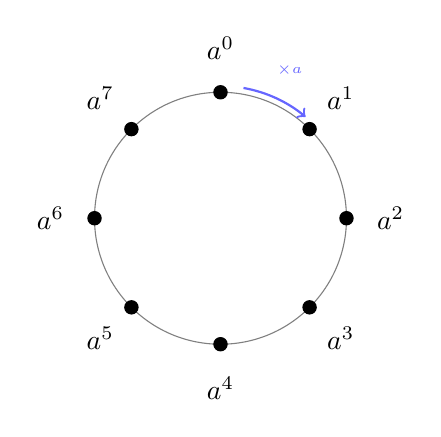
\begin{tikzpicture}[scale=1.6]
        \def\n{8}
        \draw[gray, thin] (0,0) circle (1);
        \foreach \k in {0,...,7} {
            \pgfmathsetmacro{\angle}{90 - \k * 360/\n}
            \filldraw (\angle:1) circle (1.5pt);
            \pgfmathsetmacro{\labelangle}{90 - \k * 360/\n}
            \node at (\labelangle:1.35) {$a^{\k}$};
        }
    % Arrow showing multiplication direction
        \draw[->, thick, blue!60] (80:1.05) arc (80:50:1.05);
        \node[blue!60] at (65:1.3) {\tiny $\times a$};
    \end{tikzpicture}
    \caption{Elements of a cyclic group of order $8$ on a circle}
\end{figure}

\Corollary{}{
    The order of an element $a$ in a group $G$ is the smallest positive integer $n$ such that $a^n = e$, if such $n$ exists. Otherwise, $a$ has infinite order.
}

\Example{Order of a $k$-cycle}{
    The order of a $k$-cycle $\sigma = (a_1, a_2, \ldots, a_k)$ in $S_n$ is $k$. Applying $\sigma$ repeatedly cycles each element through the $k$ positions, and after exactly $k$ applications, every element returns to its original position.
}

\Example{}{
    In $\Z_{12}$ (additive notation), the order of $3$ is $12/\gcd(12, 3) = 12/3 = 4$, and $\langle 3 \rangle = \{0, 3, 6, 9\}$. The order of $5$ is $12/\gcd(12, 5) = 12/1 = 12$, so $5$ generates all of $\Z_{12}$.
}


%%%%%%%%%%%%%%%%%%%%%%%%%%%%%%%%%%%%%%%
%  Subgroups of Finite Cyclic Groups  %
%%%%%%%%%%%%%%%%%%%%%%%%%%%%%%%%%%%%%%%

\subsubsection{Subgroups of Finite Cyclic Groups}

\Theorem{Subgroups of $\Z_n$}{
    Let $G = \langle a \rangle$ be a cyclic group of order $n$, and let $b = a^s \in G$. Then $b$ generates a cyclic subgroup $H$ of $G$ containing $n/d$ elements, where $d = \gcd(n, s)$. Moreover, $\langle a^s \rangle = \langle a^t \rangle$ if and only if $\gcd(n, s) = \gcd(n, t)$.
}

\Proof{
    By the classification theorem, $H$ has as many elements as the smallest positive integer $m$ such that $b^m = e$. Now $b^m = (a^s)^m = a^{sm}$, and $a^{sm} = e$ if and only if $n \mid sm$.

    Let $d = \gcd(n, s)$. We want the smallest $m$ such that $n \mid sm$, i.e., such that $\frac{sm}{n} = \frac{(s/d)m}{n/d}$ is an integer. Since $\gcd(s/d, n/d) = 1$ (dividing out the gcd makes them coprime), we need $\frac{n}{d} \mid m$. Thus the smallest such $m$ is $n/d$, and $|H| = n/d$.

    For the second claim: since $\langle a^s \rangle$ has $n/\gcd(n,s)$ elements and there is exactly one subgroup of each order dividing $n$ in a cyclic group, $\langle a^s \rangle = \langle a^t \rangle$ iff $\gcd(n,s) = \gcd(n,t)$.
}

\Corollary{Generators of $\Z_n$}{
    If $a$ is a generator of a finite cyclic group $G$ of order $n$, then $a^r$ is also a generator of $G$ if and only if $\gcd(r, n) = 1$, i.e., $r$ is relatively prime to $n$.
}

\Example{}{
    To find the generators of $\Z_{18}$: we need $\gcd(r, 18) = 1$. The values of $r$ with $0 \leq r < 18$ that are relatively prime to $18$ are $1, 5, 7, 11, 13, 17$. So these are exactly the generators of $\Z_{18}$.
}

\Example{All subgroups of $\Z_{18}$}{
    Since $\Z_{18}$ is cyclic, every subgroup is cyclic. For each divisor $d$ of $18$, there is exactly one subgroup of order $d$, generated by $18/d$:
    \begin{itemize}
        \item $\langle 1 \rangle = \Z_{18}$ (order 18)
        \item $\langle 2 \rangle = \{0, 2, 4, 6, 8, 10, 12, 14, 16\}$ (order 9)
        \item $\langle 3 \rangle = \{0, 3, 6, 9, 12, 15\}$ (order 6)
        \item $\langle 6 \rangle = \{0, 6, 12\}$ (order 3)
        \item $\langle 9 \rangle = \{0, 9\}$ (order 2)
        \item $\langle 0 \rangle = \{0\}$ (order 1)
    \end{itemize}
}

\begin{figure}[H]
    \centering
    \begin{tikzpicture}[node distance=1.5cm, every node/.style={font=\small}]
        \node (Z18) at (0, 3) {$\langle 1 \rangle = \Z_{18}$};
        \node (2) at (-2, 2) {$\langle 2 \rangle$};
        \node (3) at (2, 2) {$\langle 3 \rangle$};
        \node (6) at (0, 1) {$\langle 6 \rangle$};
        \node (9) at (4, 1) {$\langle 9 \rangle$};
        \node (0) at (2, 0) {$\langle 0 \rangle$};
        \draw (Z18) -- (2);
        \draw (Z18) -- (3);
        \draw (2) -- (6);
        \draw (3) -- (6);
        \draw (3) -- (9);
        \draw (6) -- (0);
        \draw (9) -- (0);
    \end{tikzpicture}
    \caption{Subgroup diagram for $\Z_{18}$}
\end{figure}

\Corollary{}{
    If $G$ is a finite cyclic group of order $n$ and $H \leq G$, then $|H|$ divides $|G|$.
}

\Proof{
    Since $G$ is cyclic, $H$ is cyclic by the earlier theorem. If $G = \langle a \rangle$ and $H$ is generated by $a^s$, then $|H| = n/\gcd(n,s)$, which divides $n = |G|$.
}

\Note{
    This result foreshadows Lagrange's Theorem, which states that $|H|$ divides $|G|$ for \textit{any} finite group $G$ and subgroup $H$, not just cyclic ones. We will see this in a later section.
}
